\section{Results} % 2 pages 
\label{sec:results}
% \begin{table*}[!h]
% \caption{The runtime of the search algorithms for different number of passes.\TODO{billy: i think we'd save space by transposing this}}
% \label{tab:runtime}
% \hskip2.3cm\begin{tabular}{|c|c|c|c|c|c|c|c|c|}
% \hline
% \textbf{}          & \multicolumn{8}{c|}{\textbf{Runtime (minutes)}}                                                                                           \\ \hline
% \textbf{Task} & \textbf{Bruteforce} & \textbf{DQN} & \textbf{PG} & \textbf{-O3} & \textbf{random} & \textbf{Greedy} & \textbf{Genetic} & \textbf{No Opt.} \\ \hline
% \textbf{3 passes}  & 4725                & 44           & 49        & 0.1          & 4725            & 19              & 150             & 0.1              \\ \hline
% \textbf{12 passes} & 3.58E+18            & 31           & 21        & 0.1          & 360             & 222             & 411             & 0.1              \\ \hline
% \textbf{24 passes} & 2.46E+38            & 20           & 34        & 0.1          & 360             & 837             & 1017            & 0.1              \\ \hline
% \end{tabular}
% \end{table*}
% The algo shown in Fig 7 takes 1025mins to for 3 passes on 4 progs 
% 
\vspace{-0.1cm}
We implemented the framework in Python and TensorFlow~\cite{TF}. The network topology consisted of a $512\times256$ FC layer for the DQN, and $256\times256$ FC layer for the PG. We ran the framework on a four-core Intel i7-4765T CPU~\cite{Intel2017} with a Tesla K20c GPU~\cite{Nvidia2012} for handling the training and inference.
We use the number of clock cycles reported by the HLS profiler as the performance metric. 
In~\cite{huang2013effect}, results showed a one-to-one correspondence between the clock cycle count and the actual hardware execution time. Therefore, better clock cycle count will lead to better hardware performance. 
%We also validated the reported clock cycles with logic simulation. 

%Moreover, the clock cycle counts can be reported during the compile time within seconds, which allows us to generate adequate number of trajectories for RL\TODO{Ameer: Do we need this sentence? }. 
Success is defined as learning a sequence of passes that performs better than -O3 within a reasonable time. 
%This is mainly due to a compile time constraint imposed by the deep reinforcement learning algorithms. 
%The clock cycle counts can be reported by the HLS profiler during the compile time within seconds. 
%(which minimizes the number of cycles) based on the features extracted from the program. 
We use $12$ benchmarks for evaluation taken from CHstone~\cite{hara2008chstone} and LegUp examples. The benchmarks contain a variety of applications from different domains, such as arithmetic, media, and cryptography. The number of cycles required to run the benchmarks ranges from thousands to millions. We ran DQN and PG, and compared it against random search, greedy algorithms~\cite{huang2013effect}, genetic algorithms~\cite{DEAP_JMLR2012}, and -O3. All results are normalized to the case where no optimization was applied.
%It is written in a limited subset of standard C excluding the structures that are not commonly supported by the HLS tools, such as floating-point, struct composition, dynamic memory allocation and recursion. 
%All programs in the CHStone benchmark suite are synthesizable.

\subsection{Impact of the Sequence Length}
Figure \ref{fig:length} shows the circuit speedup for various algorithms with sequence lengths of 3, 12, and 24.  
For each algorithm, we set the optimization sequence to a fixed length.
The sequences for three passes are generated with each algorithm running to optimize for four programs. 
The sequences for 12 and 24 passes are generated with each algorithm optimizing six programs. 
We then applied the generated sequences to all 12 programs, normalized the results to the No-Opt performance, and  
took the average of the normalized performance for the 12 programs. 
Results show that three passes is not adequate to achieve peak performance for the 12 benchmarks. 

For DQN, PG, genetic and greedy algorithms, little performance improvement is observed by increasing the length from 12 to 24. 
With 24 passes, PG, DQN and Genetic algorithms perform better than the rest. 


%\subsection{3 Passes}
% \begin{figure*}[!t]
%     \centering        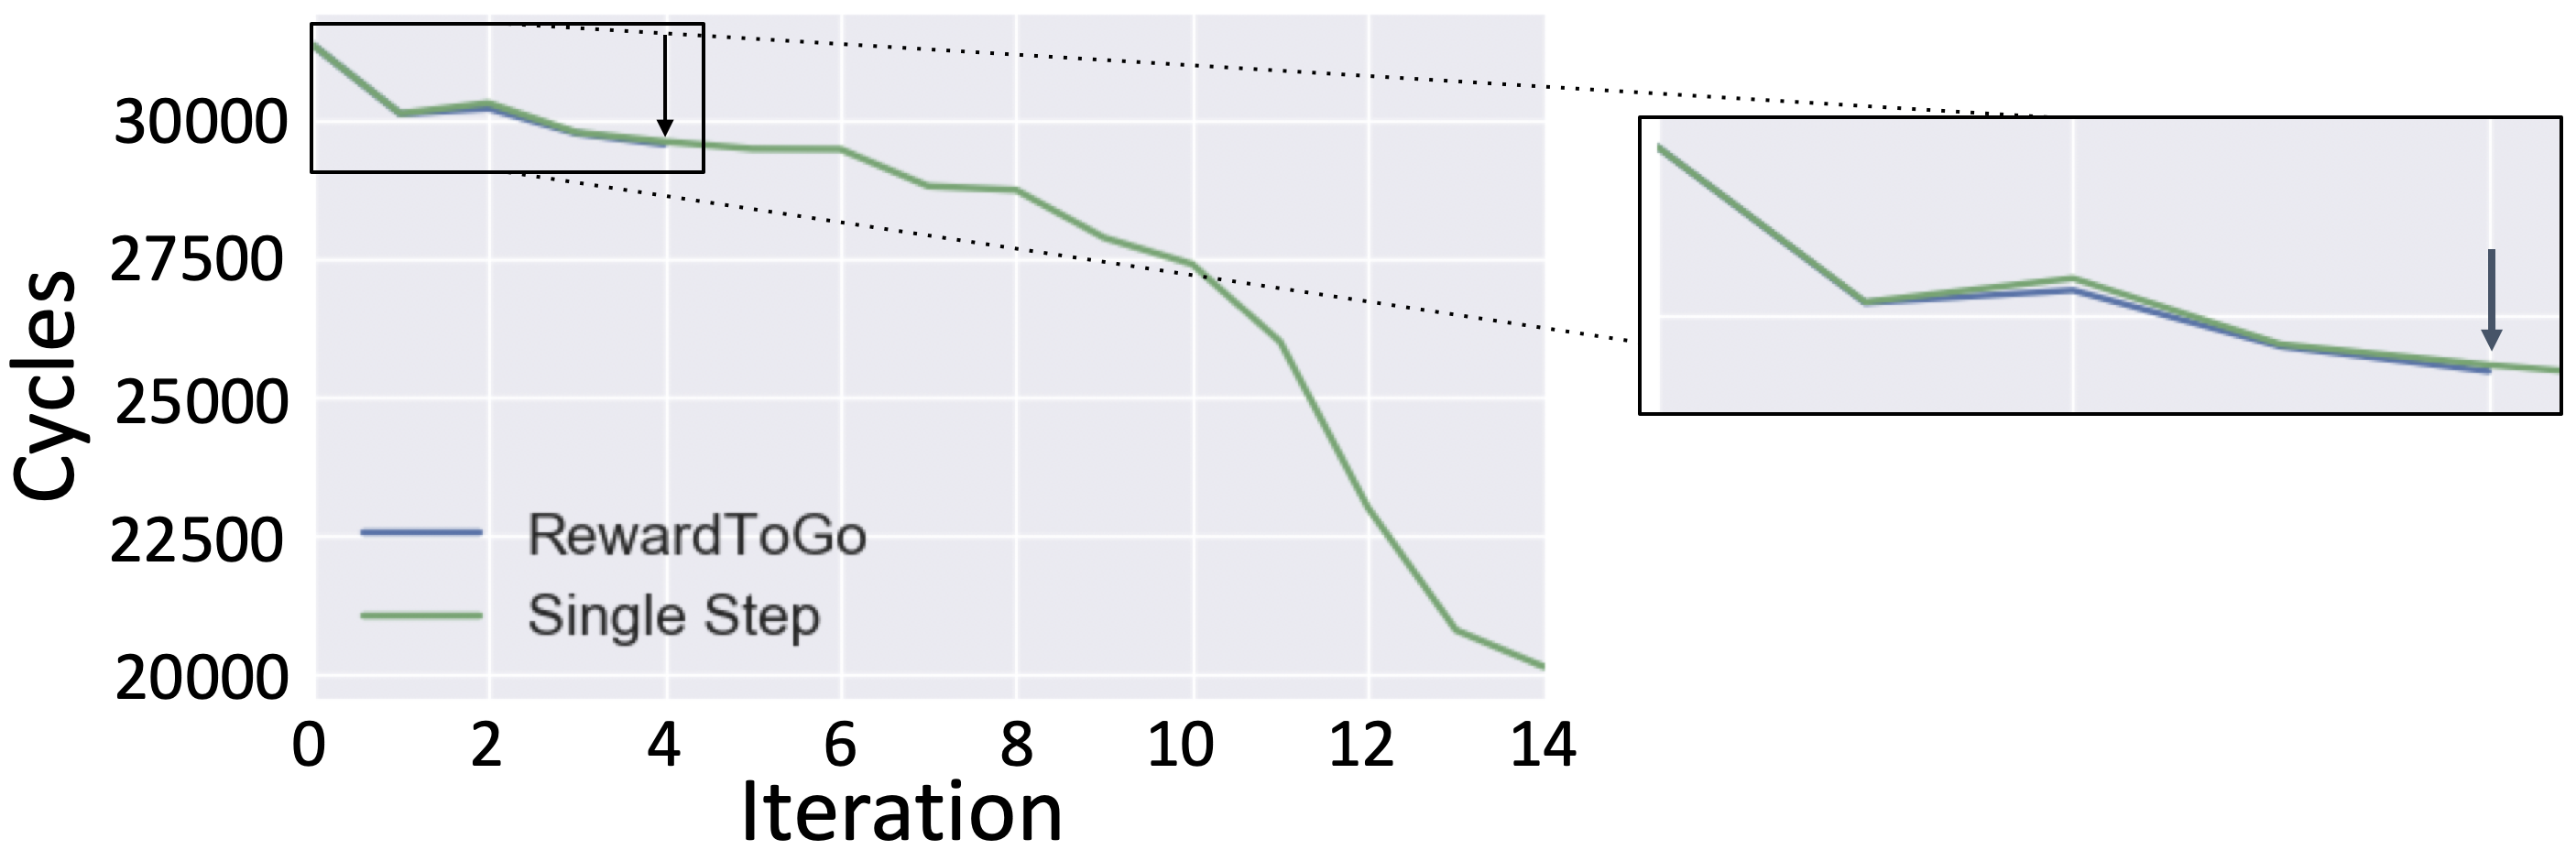
\includegraphics[width=\textwidth]{Figures/PG3passv2.png}    
%     \caption{The mean cycles as a function of timestep in the PG framework to find the three optimal passes.}
%     \label{fig:PG1}
% \end{figure*}

% \begin{figure}[!t]
%     \centering
%     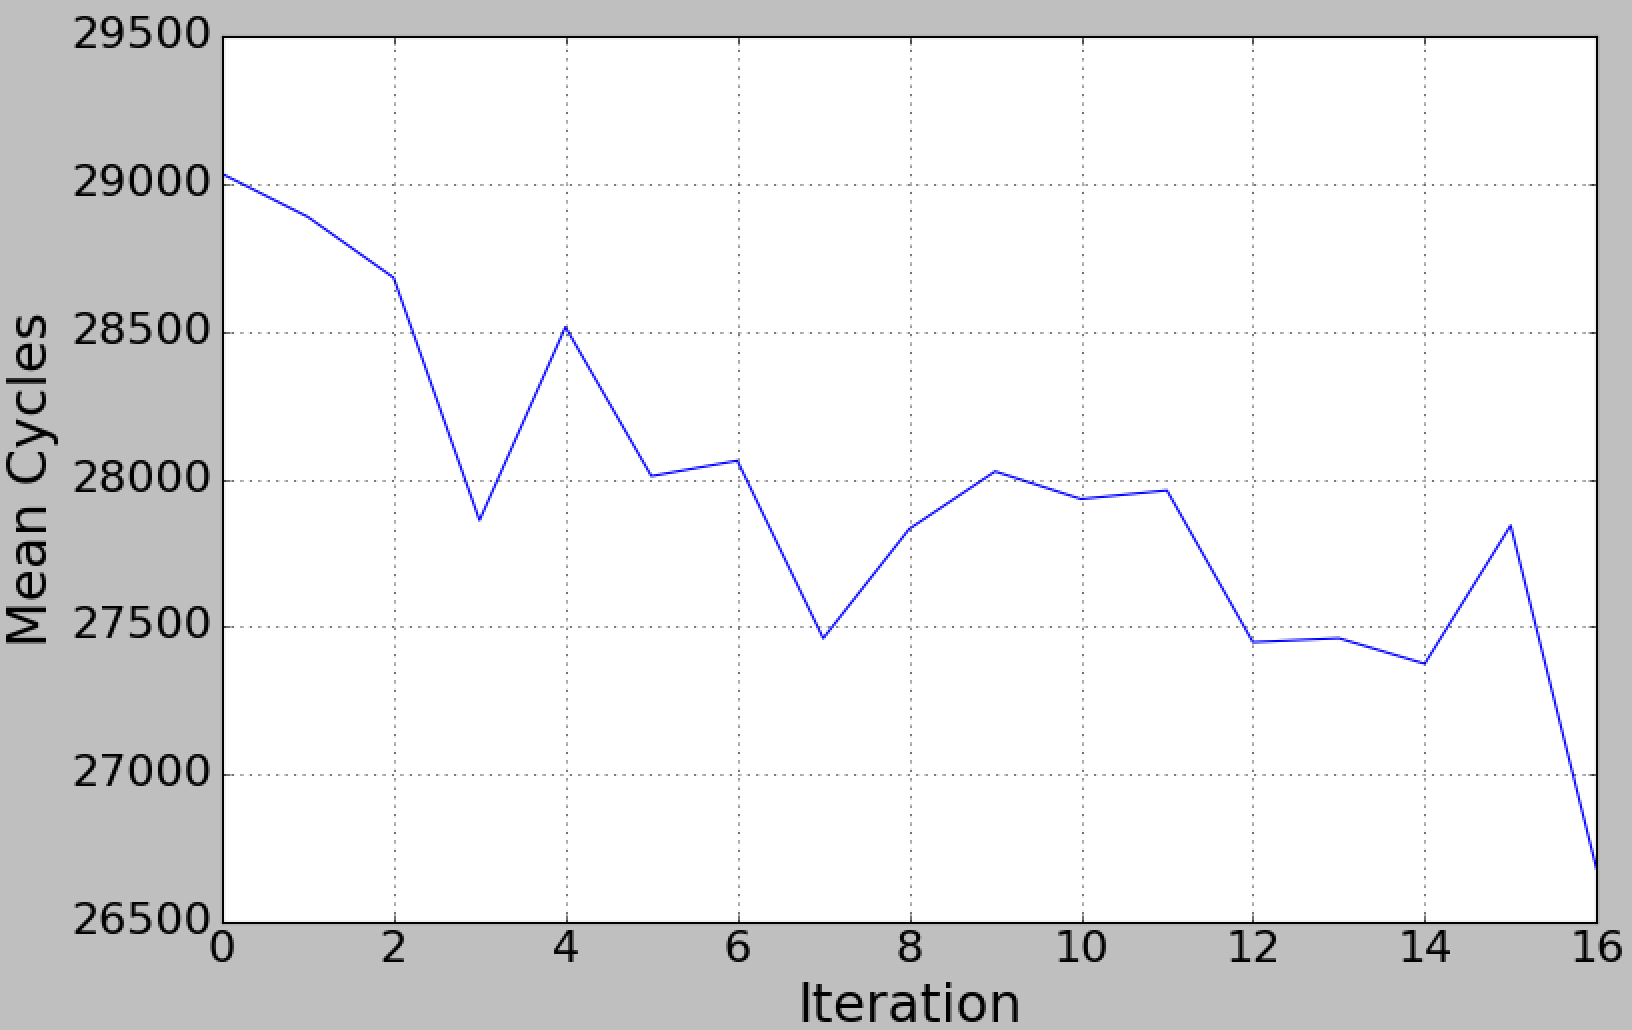
\includegraphics[width=0.5\textwidth]{Figures/dqn3pass.png}
%     \caption{The cycles as a function of timestep in the DQN framework to find the three optimal passes.}
%     \label{fig:dqn1}
% \end{figure}
%Our first evaluation is to evaluate the performance of the different search algorithms with a small number of passes
\begin{table}[!t]
\caption{The optimization time of the search algorithms for different number of passes.}
\vspace{-0.2cm}
\label{tab:runtime}
\begin{tabular}{|c|c|c|c|c|c|c|}
\hline
\textbf{}          & \multicolumn{6}{c|}{\textbf{Optimization Time (minutes)}}                                                                                           \\ \hline
\textbf{\hspace{-1.2mm}\# passes\hspace{-1.2mm}} & \textbf{\hspace{-1.2mm}Exhaustive\hspace{-1.2mm}} & \textbf{\hspace{-1.2mm}DQN\hspace{-1.2mm}} & \textbf{PG} & \textbf{\hspace{-1.2mm}Random\hspace{-1.2mm}} & \textbf{\hspace{-1.2mm}Greedy\hspace{-1.2mm}} & \textbf{\hspace{-1.2mm}Genetic\hspace{-1.2mm}} \\ \hline
\textbf{3 passes}  & 4725                & 44           & 49                & 4725            & 19              & 150                       \\ \hline
\textbf{12 passes} & 3.58E+18            & 31           & 21                & 360             & 222             & 411                      \\ \hline
\textbf{24 passes} & 2.46E+38            & 20           & 34             & 360             & 837             & 1017                    \\ \hline
\end{tabular}
\vspace{-0.5cm}
\end{table}

\subsection{Optimization Time Comparison}

Table~\ref{tab:runtime} lists the time it took to run each algorithm for differing number of passes. For three passes, it is possible to find the optimal sequence as the exhaustive-search is feasible. The exhaustive-search solution took $78.75$ hours to run. We ran the random search for $78.75$ hours, yet it did not find the optimal sequence. Also the greedy algorithm did not find this sequence.


The DQN, PG, and genetic algorithms quickly achieved this sequence. Additionally, DQN and PG achieved this sequence $3.4\times$ and $3.1\times$, respectively, faster than the genetic algorithm. To ensure  RL did not achieve the sequence by luck, we ran the RL framework ten times and verified that it derived the optimal ordering every time. Furthermore, we kept running the RL until it found the optimal sequence, although it found suboptimal ones much earlier. This is why it took more time to run the RL frameworks with three passes.
The optimal sequence was \textit{-simplifycfg, -loop-rotate}, and \textit{-loop-unroll}. Note that even with $3$ passes the performance of RL is 1.5\% better than -O3.
%For simplicity, we run the algorithms on four programs rather than twelve as these passes are optimal for most tasks. 
%Because of this, 
%The performance of the programs for the different search algorithms is shown in Figure~\ref{fig:3pass}. 
%By contrast, 

Results show that adding more passes resulted in a minor impact on optimization time for the RL algorithms but a major impact for the greedy and genetic algorithms. Note that for 12 and 24 passes, it would take more than one trillion years to run exhaustive-search. Therefore, the time given is an estimate based on the optimization time for three passes. Furthermore, we limited the time to run random search to six hours when applying 12 and 24 passes. Greedy and genetic algorithms run one to two orders of magnitude slower than the RL algorithms and achieve lower circuit performance for greedy algorithm and similar circuit performance for genetic algorithm. The algorithm optimization time benefits are mainly due to the data efficiency of the RL algorithms and the optimizations proposed in Section~\ref{sec:DRLA} that make it possible to significantly reduce the number of compilations required when running the framework and using the previously applied passes as the input observations. %The optimal sequence it arrived at was \textit{-sink, -loop-rotate}, and \textit{-loop-unroll}.  %which achieves 3.5\% lower performance than the optimal. Note that even with $3$ passes the performance of RL is 1.5\% better than -O3. The performance of RL is also 10\% better than greedy. The genetic algorithm was able to achieve similar results but in $3\times$ longer time. The runtimes are summarized in table~\ref{tab:runtime}. 

\begin{figure}[!t]
    \centering
    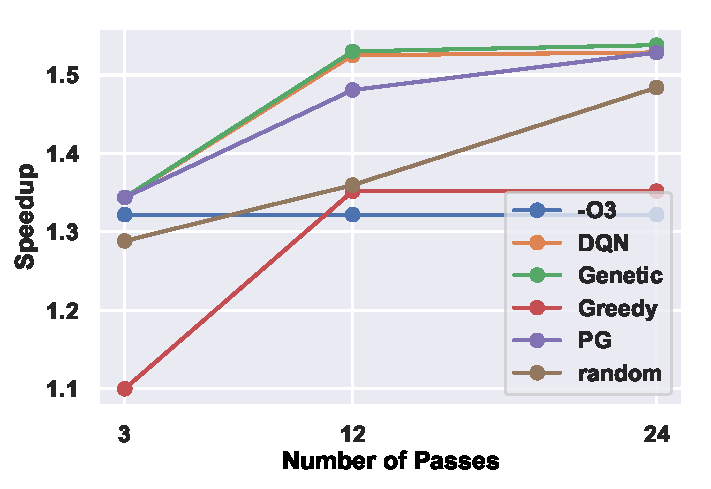
\includegraphics[width=0.5\textwidth]{Figures/length.pdf}
    \vspace{-0.7cm}
    \caption{Circuit speedup of various algorithms compared to No-Opt with sequence length of 3, 12, and 24.}
    \label{fig:length}
    \vspace{-0.5cm}
\end{figure}

% Figure~\ref{fig:PG1} shows the number of cycles as a  function of timestep for the PG algorithm. The graph shows two plots, one for the PG algorithm (Single Step) where we only compile once at the end of the roll-out and another (RewardToGo) for the PG algorithm where we compile once after each pass applied and use the reward to go~\cite{Baxter2001} to reduce variance and thus further improve its performance. Within the same time frame, it is evident that since we are optimizing three passes, the runtime improves by $3\times$ when using Single Step over RewardToGO and the performance it achieves is $40\%$ better performance. 
\begin{figure*}[!t]
    \centering        
    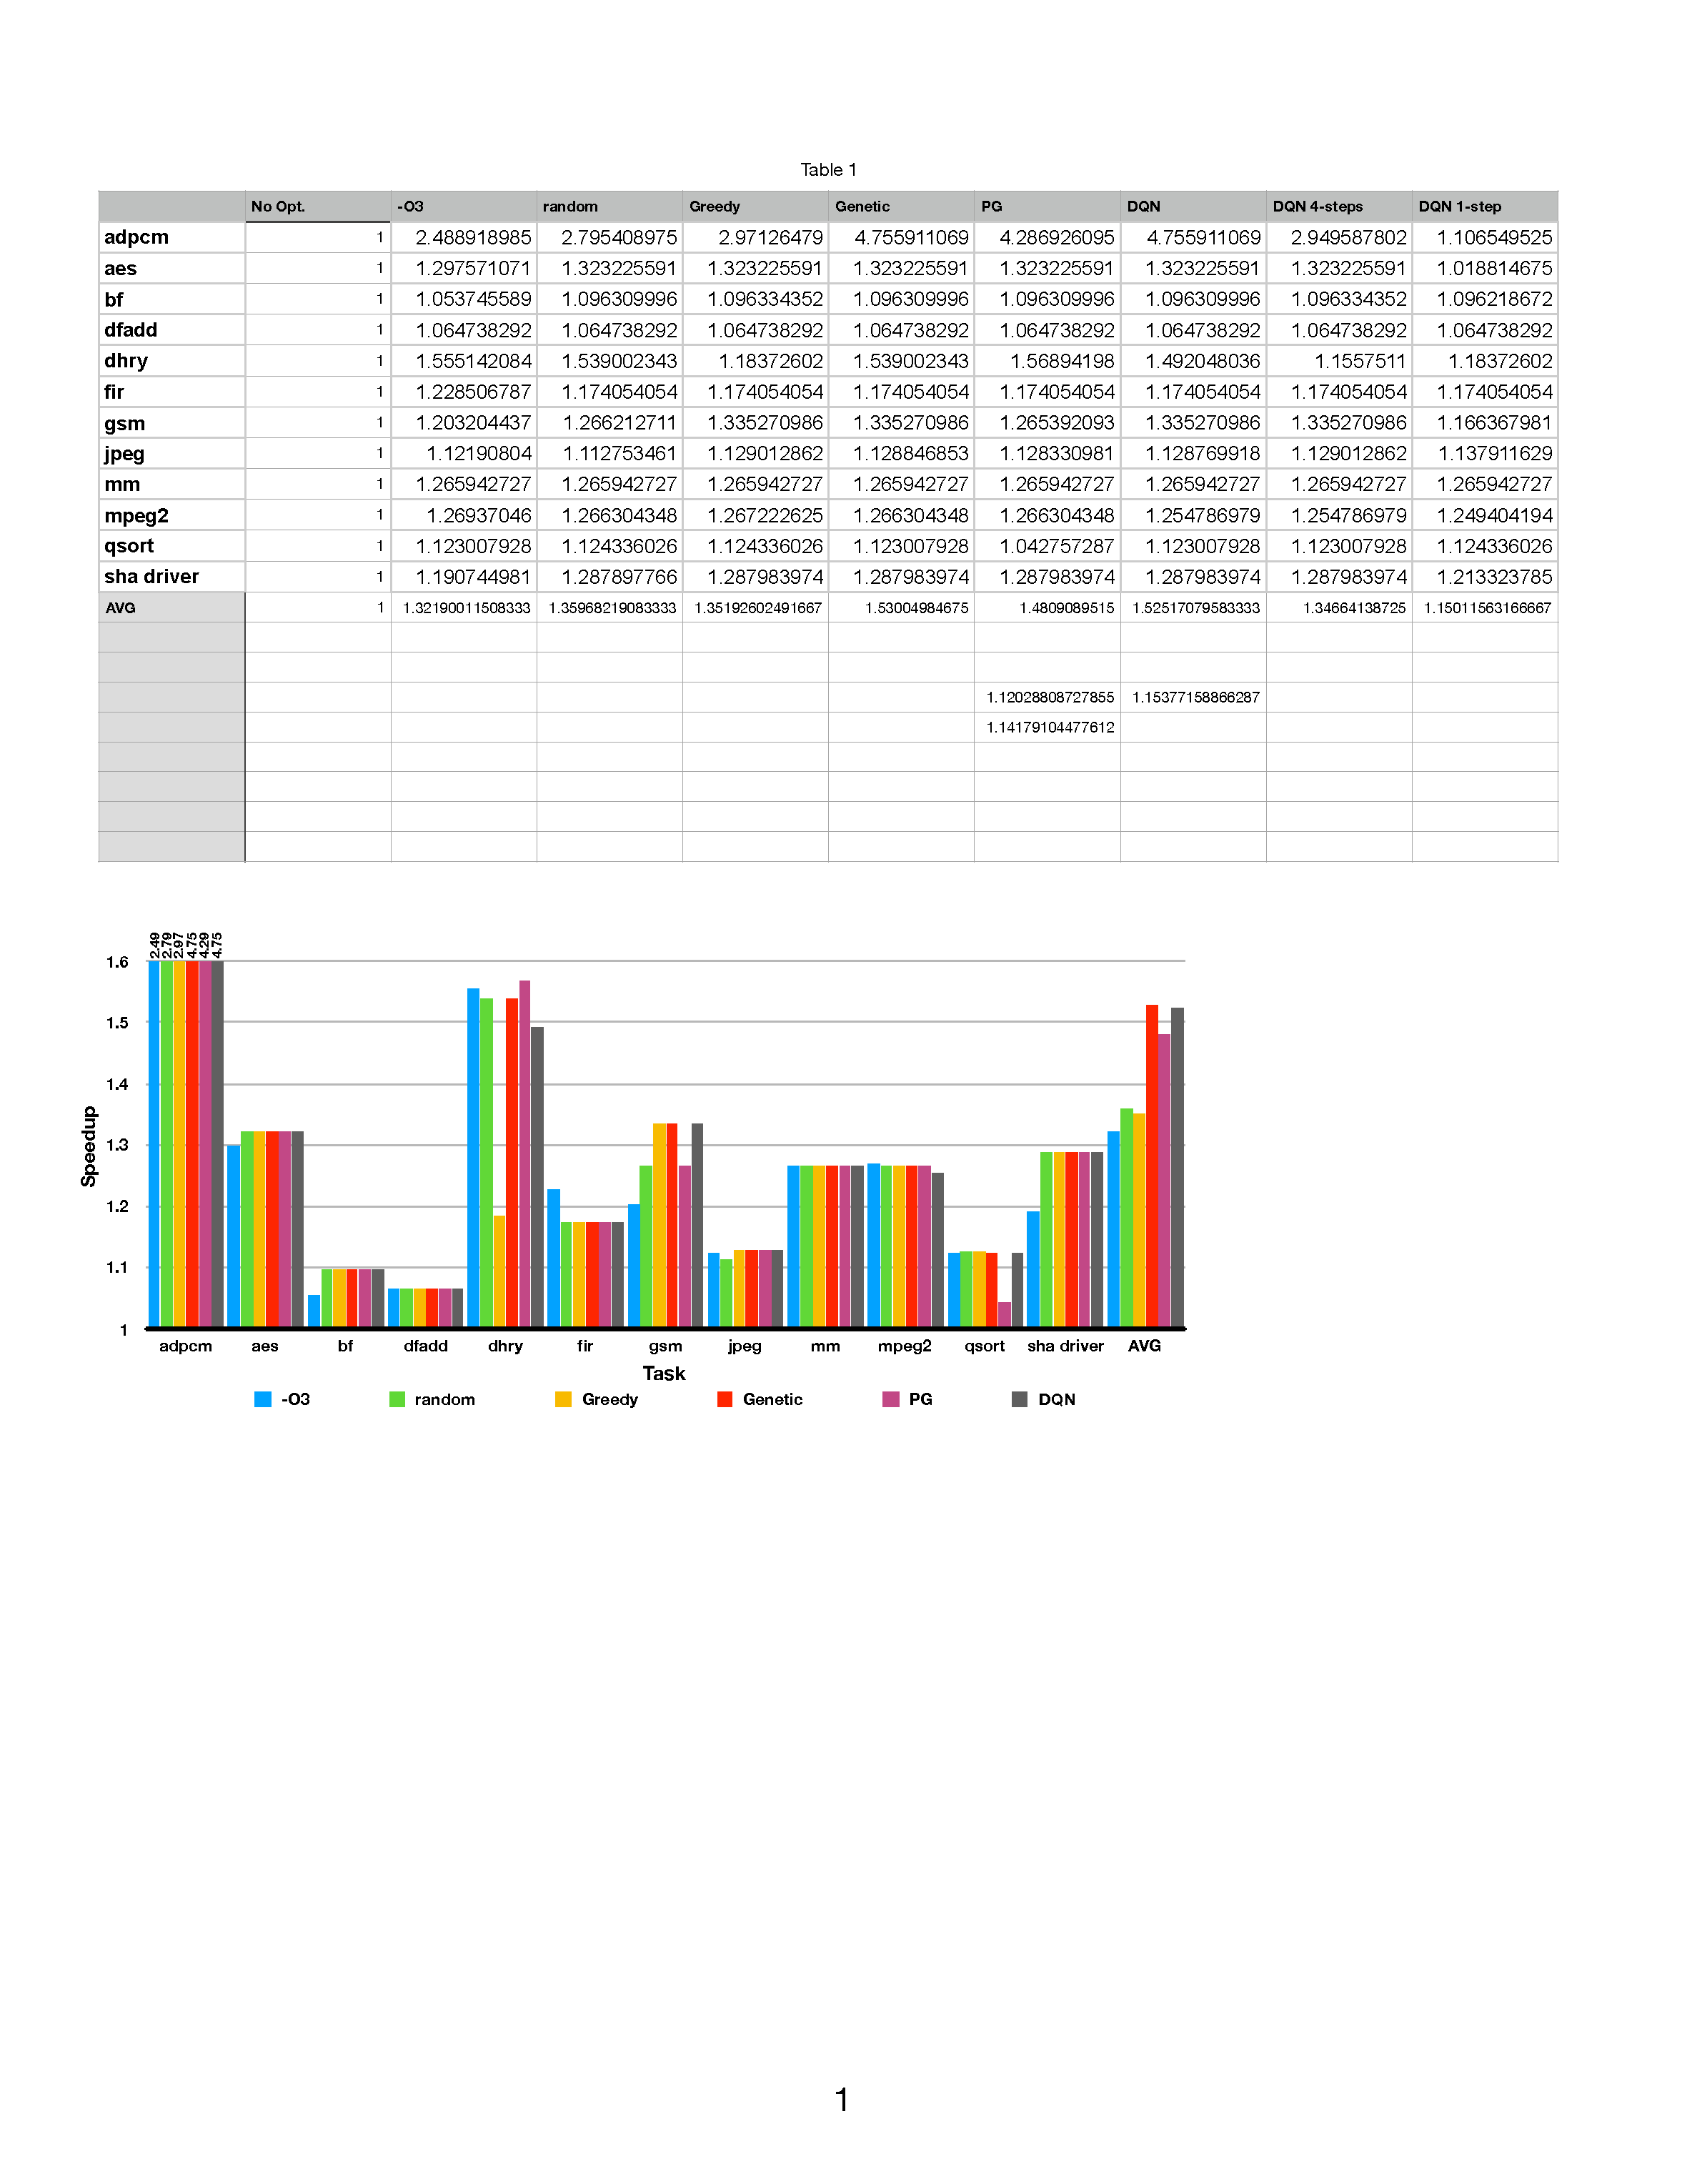
\includegraphics[trim={1.9cm 18cm 11.5cm 21.5cm},clip,width=\textwidth]{Figures/12passesv5.pdf} 
    \vspace{-0.7cm}
    \caption{The circuit speedup for searching the best 12 passes using the different search algorithms for different tasks normalized to the case without any optimization.%The exact number of cycles are listed in the appendix in Table~\ref{tab:12pass}
    }
    \label{fig:12pass}
    \vspace{-0.6cm}
\end{figure*}


% Figure \ref{fig:dqn1} shows the mean number of cycles as a function of timestep for the DQN algorithm. DQN runs much faster than PG. In all of our runs DQN found the optimal solution but it did not always stabilize there. But since we care only about a single good roll-out it was sufficient.

%\subsection{12 Passes}
\vspace{-0.1cm}
\subsection{Circuit Performance Comparison}
\vspace{-0.1cm}

Figure~\ref{fig:12pass} shows the circuit speedup of the different algorithms for finding the best $12$ passes as a function of time, normalized to No-Opt performance. The highest improvement is seen in DQN and genetic algorithms that both achieve $16\%$ better circuit speed over -O3 (six programs improved, three programs remained the same, and three programs worsened slightly). PG achieves $12\%$ better circuit speed over -O3. DQN requires less data to learn and this is why it achieves better speedup over PG. 
%Random search achieves slightly higher speedup than -O3, and greedy. This is mainly because we run it for a longer time and it runs more samples over time, as no training/processing is required on the data.


Figure~\ref{fig:12vstime} shows the geomean of circuit cycles of the programs as a function of time for genetic and greedy algorithms, and the average geomean of cycles for PG and DQN (averaged over batch size). For a fair comparison we cut the time after the algorithms stop improving. 
The greedy and genetic algorithms both have a large improvement at the beginning of the training phase because of its greedy nature. 
The greedy algorithm converges to a worse minimum result compared to the other algorithms, suggesting locally optimal choices may not be the best approach for tackling the phase-ordering problem. 
The genetic algorithm, however, has mutation, introducing randomness which helps to improve the performance. 
We see that both RL algorithms improve the average cycles of a batch over time. 

\subsection{Validation}
\vspace{-0.1cm}
After the framework finishes running on the LegUp simulator, we validate the cycle time results by compiling the generated Verilog and simulating the design with ModelSim. 
We see a 0.48\% difference between the actual and profiler-generated cycle time. 
We also compile all the optimized circuit designs with a standard FPGA toolflow and verify that frequency meets the 50 MHz constraint. We take the geomean across all the benchmarks for the area results. Compared to the -O3 area results, the DQN-optimized circuits have 0.6\%, 3\%, 43\% increase in LUTs, registers, and BRAMs respectively. The DSPs remained the same. Note that the objective of this paper is to optimize for circuit speed. Optimizing for area or both circuit speed and area is also feasible in a similar manner.
%\TODO{add area disimprovement}. 
%We now increase the number of passes to $12$. Note that a brute force solution would take more than one trillion years to run in that case. To see how well it scales we train on six programs and use these results to compile $12$ programs. The performance of the programs for the different search algorithms is shown in Figure~\ref{fig:12pass}. The runtimes are summarized in table~\ref{tab:runtime}. Three DQN results are presented: DQN $n$-steps where we compile once after applying $n$ passes and average the reward for $n=1,4,12$.  The highest performance is achieved in DQN $12$-steps and genetic algorithms that both achieved 16\% better performance than -O3, genetic, random and PG algorithms. Furthermore, DQN $12$-steps runs $7.1\times$ and $63\times$ faster than the greedy and genetic algorithms respectively. PG runs $10.5\times$ faster than greedy algorithms while achieving similar performance. 

\begin{figure}[!t]
    \centering
    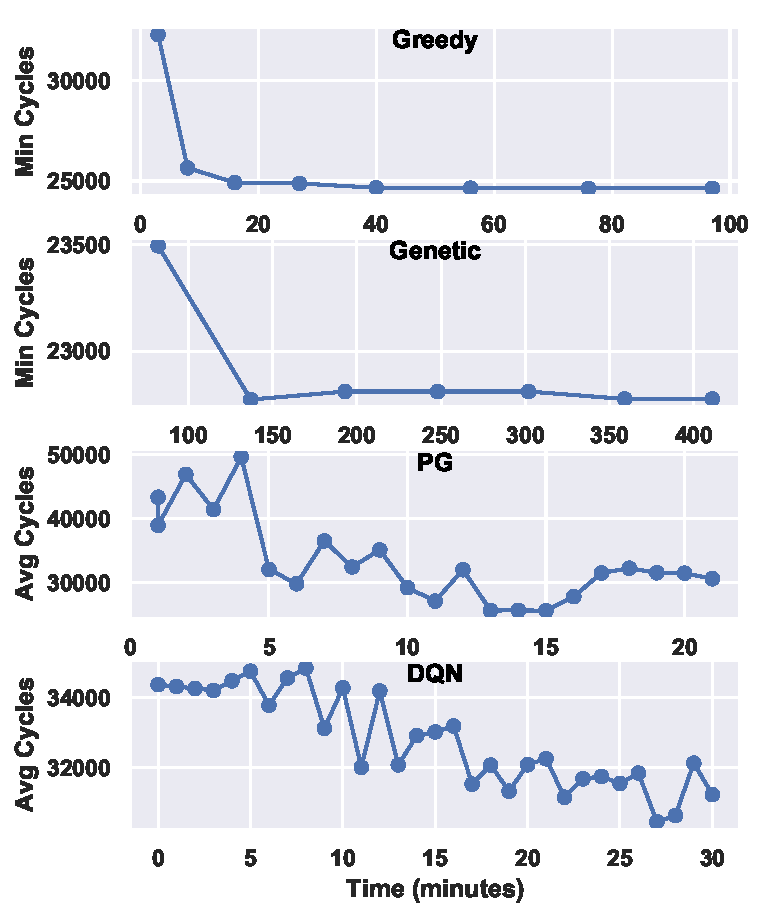
\includegraphics[trim={0cm 0cm 0cm 0.3cm},clip,width=0.5\textwidth]{Figures/12vstime.pdf}
    \vspace{-0.7cm}
    \caption{Geomean of circuit cycles for various algorithms as a function of algorithm training time.}
    \label{fig:12vstime}
    \vspace{-0.5cm}
\end{figure}

%\subsection{Impact on Generated Hardware}
%Table shows the actual cycle time of the programs. 
%\JENNY{Add tables}
%\subsection{Challenges and Discussion}
% \subsubsection{DQN $n$-steps}
% Figure~\ref{fig:dqn2} shows the mean cycles as a function of time step for the three DQN approaches. DQN $12$-steps is able to run more trajectories, explore more, take advantage of a larger batch size and find better results. On the other hand, it suffers from higher variance than DQN 4-steps and DQN 1-step, because the accuracy of the reward decreases when averaging over larger group of passes. DQN 4-steps  takes advantage of both exploration and lowered variance, but still achieves worse performance than DQN $12$-steps as it runs less trajectories in the same time frame. After running it for 15 additional minutes DQN $4$-steps achieved similar performance results to that of DQN $12$-steps. DQN $1$-step on the other hand has the least variance but since it runs very slow it explores less and requires much more time to run.

% \begin{figure}[!t]
%     \centering
%     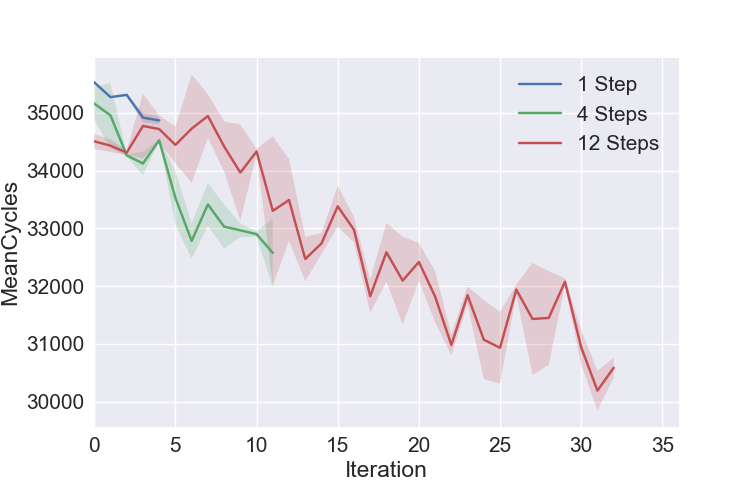
\includegraphics[width=0.5\textwidth]{Figures/dqn12pass.png}
%     \caption{The means cycles as a function of timestep in the DQN framework to find the $12$ optimal passes.}
%     \label{fig:dqn2}
% \end{figure}
% \subsubsection{PG vs. DQN}
% DQN is known to be more data efficient that PG \textit{i.e.,} require fewer samples than PG to learn. This is why DQN achieved better results than PG in similar time frames. Furthermore, DQN has more randomness/exploration part that allows it to explore more. Interestingly, the random search on $12$ passes achieved similar performance as PG, greedy and -O3 algorithms (although it took longer time to run). Given the large exploration space, the higher level of randomness in DQN gave it additional performance benefits.

% \subsubsection{Reward-to-go}     
% \begin{figure}[!t]
%     \centering
%     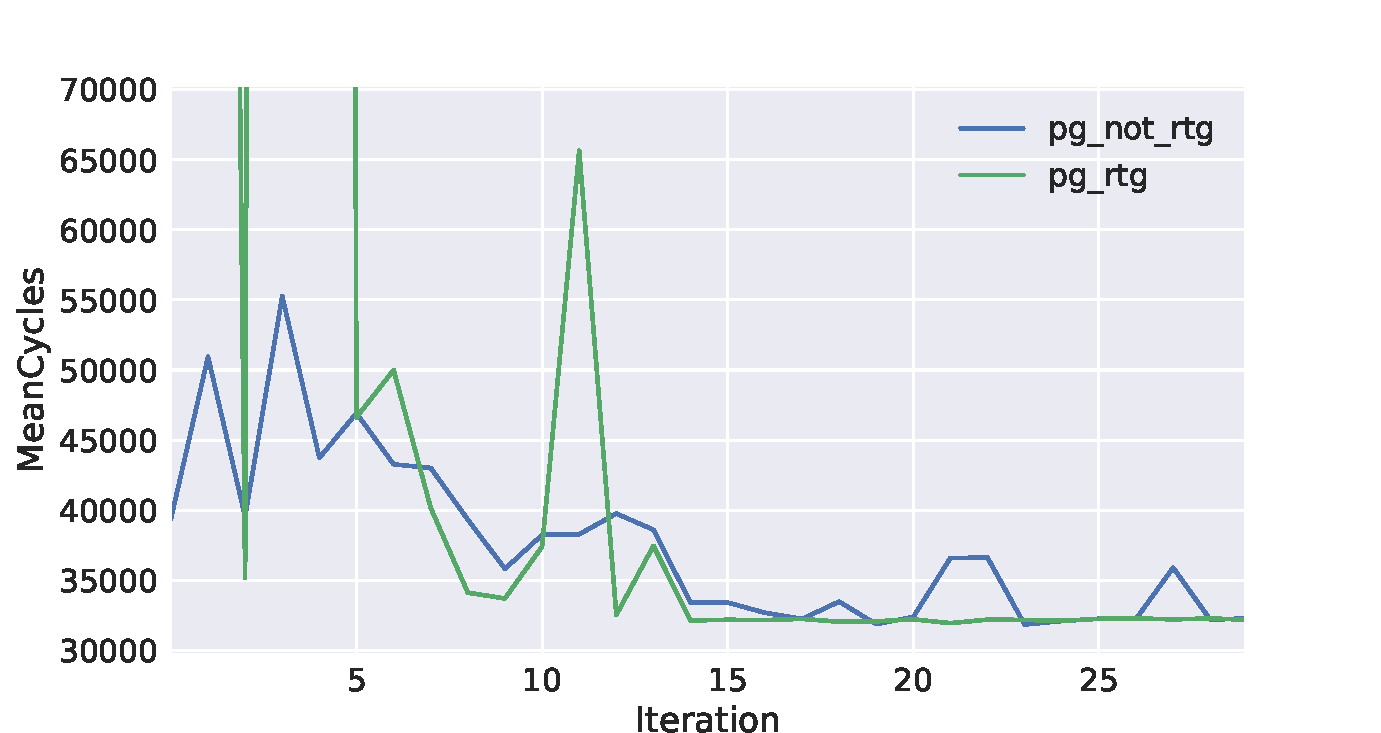
\includegraphics[width=0.5\textwidth]{Figures/pg_rtg_meancycle.pdf}
%     \caption{Mean Clock Cycles versus Training Iterations for Policy Gradient algorithms with and without Reward-to-go for a batch size of 100.}
%     \label{fig:pg_rtg}
% \end{figure}
% We run an experiment to compare the policy gradient with and without the use of reward-to-go for the $12$ passes with a batch size of 100. 
% %Instead of only running the simulator environment once after each trajectory with a fixed length is generated for reward estimation, we need to run the simulator environment every time after we apply a new pass to gather rewards for the neural network to learn the reward-to-go value function.
% While there is no significant difference in the final number of clock cycles shown in Figure~\ref{fig:pg_rtg} for both algorithms. Adding reward-to-go results in $11\times$ longer runtime (21 minutes vs 253  minutes). Thus, reward-to-go is not adopted in our algorithm to save the training time. 
% \subsubsection{PG Batch Size Sensitivity Analysis}
% Figure~\ref{fig:pg_batch} shows the learning curve of the policy gradient method with three different batch sizes: 100, 200 and 500. 
% We can see that the policy gradient converges to a lower minimum with larger batch sizes.
% However, the runtime of the algorithm for the same number of training iterations increases with the batch size. The training time is 21 minutes, 41 minutes and 103 minutes respectively. 

%\subsubsection{Trajectory}
%The maximum trajectory length used in this work is $12$ passes. This is due to the limited resources and time to generate the results that consume time which increases exponentially with the number of passes applied. Nevertheless, we ran some experiments of up to $96$ passes and realized the performance improvements in all the algorithms is up to 3\% in the best case while the runtime could extend to multiple days. We also tried using -O3 as a pass that the RL can choose to apply, but the results did not change.

\subsection{Possible Alternative Machine Learning Algorithms}
\vspace{-0.1cm}
Inspired by the observed advantage of randomness in random search, genetic algorithm, and DQN that enables more exploration, as well as the redundancy of observations, we believe other techniques such as Bandits~\cite{chapelle2011}, Exploration~\cite{bellemare2016}, Proximal Policy Gradients~\cite{schulman2017proximal}, and Evolution Strategies~\cite{salimans2017evolution} might also be good candidates to explore. These works leverage a great deal of randomness and exploration while maximizing rewards. Furthermore, it might be beneficial to combine the applied optimizations and program features as observations to the RL so it could benefit from both representations of the state.
% \begin{figure}[!t]
%     \centering
%     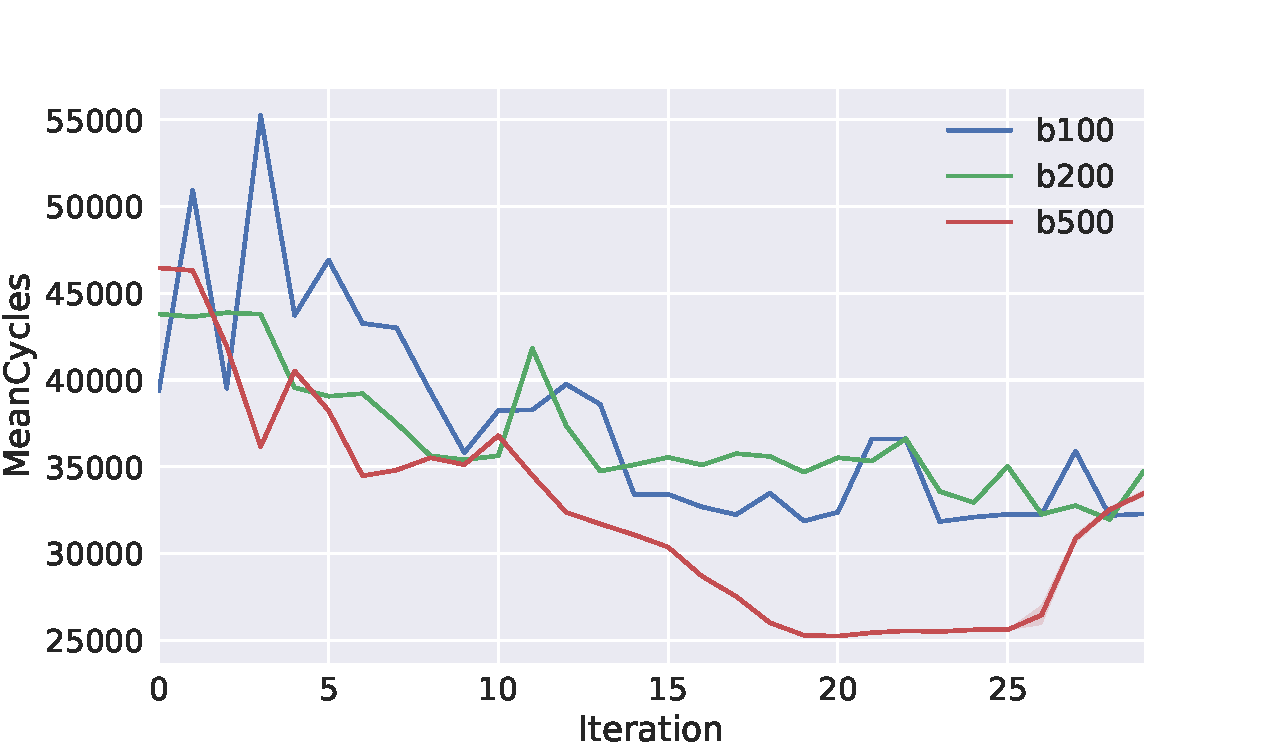
\includegraphics[width=0.5\textwidth]{Figures/pg_batch_meancycle.pdf}
%     \caption{Mean Clock Cycles versus Training Iterations for Policy Gradient algorithms with different batch sizes.}
%     \label{fig:pg_batch}
% \end{figure}
%\item Comparison among different ML algorithms 
%    \subitem put the table from midterm report 